\documentclass[11pt]{article}
\usepackage[margin=0.93in]{geometry}
\usepackage{amsmath,amssymb,graphicx}
\usepackage[hidelinks]{hyperref}
\newcommand{\E}{\mathbb E}
\newcommand{\one}{\mathbf 1}
\newcommand{\diag}{\mathop{\rm diag}}
\newcommand{\Rea}{\mathop{\rm Re}}
\setlength{\parindent}{1em}
\setlength{\parskip}{2pt}
\setlength{\emergencystretch}{1.5em}
\title{Optimal detector memory under stochastic resetting: a nine-stage threshold and a bound on its benefit}
\author{}
\date{27 November 2026}
\begin{document}
\maketitle
\begin{abstract}
A particle passes a detector once per excursion. At Poisson reset times the particle returns to its source, while the detector either retains its state or draws a fresh one from stationarity. When can a mixture of these two policies minimize the mean detection time? For a homogeneous driven three-state detector and a flight composed of independent exponential stages, eight or fewer stages exclude a strict interior optimum. Nine suffice at finite cycle affinity. The criterion follows from the phase of the flight-time Laplace transform evaluated at a complex relaxation rate. More generally, the change in mean detection time is a weighted open-state autocovariance, so retention strictly slows detection for every reversible finite gate in this model. For a driven twelve-state gate, full retention reduces the mean by 1.87\% in a ballistic example. For a growing biased ring we resolve a sign change on the scale of inverse ring size in the refresh probability. For the three-state gate, the fractional advantage of any mixed policy over the better endpoint is uniformly below 0.01014\% for independent exponential stages, even with unequal rates. The same bound holds for deterministic flights.
\end{abstract}

\section{One encounter per excursion}
A sensor at a fixed point records a passing particle only when an internal gate is open. A missed particle travels on until a reset returns it to its source. Resetting the apparatus may also erase the phase of the gate. If the gate runs around a driven cycle, a missed passage contains information about the phase at a future passage. Does erasing this information speed up or delay detection?

Studies of gated diffusion distinguish resetting both particle and gate from resetting position alone \cite{bress,mercado,biswas}. Renewal methods relate gated reactions to first encounters and returns \cite{scher}; hitting times for chains with probabilistic restart have a broader theory \cite{avra}. A blinking-target model also allows a closed target to be crossed and revisited after a miss \cite{zbik}. Here an excursion has one opportunity to detect. A reset can pre-empt that opportunity or occur after a miss, and the intervening time changes the phase presented to the next excursion. Our control variable is the probability of retaining that phase at a fixed reset rate. The contrast between an equilibrium and a driven detector follows from a return correlation of the free gate. The sharp stage threshold below concerns the joint dependence on gate drive and travel-time dispersion.

At launch the particle draws an independent flight time $S$, with $0<S<\infty$ almost surely. Ballistic travel over distance $L$ at speed $v$ gives $S=L/v$. A directed sequence of $n$ independent exponential transit stages gives an Erlang time when the rates are equal. There is one instantaneous detection test at age $S$ if no reset has intervened. A closed gate is transparent. A Poisson clock of rate $r>0$ resets the particle regardless of its position. On reset, independently retain the current gate with probability $c\in[0,1]$ and otherwise redraw it from stationarity. The flight time, reset clock, and free gate noise are independent. Each flight starts afresh. The initial gate is stationary; the gate among surviving trajectories generally is not.

\section{Mean time in terms of the free detector}
Let $Q$ be the row generator of a finite irreducible continuous-time chain with at least two states, $P_t=e^{Qt}$, stationary row $\pi$, and a single open state $o$. Write $e_o$ for its unit column, $p=\pi_o$, $\Pi=\one\pi$, and $L(s)=\E e^{-sS}$. The mean time to detection starting from stationarity is $T(c)$. Define the tilted flight time $S_r$ by $\Pr(S_r\in ds)=e^{-rs}\Pr(S\in ds)/L(r)$.

\paragraph{Proposition 1.} With $A(t)=(P_t)_{oo}-p$,
\begin{align}
 T(0)&=\frac{1/[pL(r)]-1}{r}, \label{eq:base}\\
 T(c)-T(0)&=\frac{c}{p}\int_0^\infty
 e^{-r(1-c)t}\,\E A(S_r+t)\,dt . \label{eq:main}
\end{align}
The integral converges also at $c=1$ because the free gate mixes exponentially. Here $pA(t)$ is the stationary autocovariance of the indicator of the open state.

\paragraph{Proof.}
The vector of successful-excursion probabilities from specified starting states is $h=\E[e^{-rS}P_S]e_o$, with $\bar h=\pi h=pL(r)$. At an independent reset epoch the freely evolving gate has kernel $B=r(rI-Q)^{-1}$. Continue every successful path as a fictitious free gate from state $o$ until that epoch. By the exponential residual waiting time, the matrix of failed excursions observed immediately before reset is $B-h e_o^\top B$. The post-reset kernel is $K=cI+(1-c)\Pi$. Put $H=BK$ and $M=(I-h e_o^\top)H$. Each $h_i$ is strictly positive, so the survival matrix $M$ has maximum row sum strictly less than one.

The expected excursion duration is $(\one-h)/r$ by integrating survival up to the independent reset. Thus the conditional mean column $u$ satisfies $ru=\one-h+Mru$. For $N=\one+ru$ this becomes $N=\one+MN$. Multiplying by $\pi$ gives $e_o^\top HN=1/\bar h$. Centering the same equation yields
\[
 (I-H)(N-\one\pi N)=-(h-\bar h\one)/\bar h .
\]
On centered columns $H=cB$. Consequently $\pi N=[1+e_o^\top cB(I-cB)^{-1}(h-\bar h\one)]/\bar h$, where the inverse acts on centered columns only. On this space $cB(I-cB)^{-1}=cr[r(1-c)I-Q]^{-1}$. The integral representation of this resolvent and $P_tP_s=P_{t+s}$ give (\ref{eq:base})--(\ref{eq:main}). \hfill$\square$

\section{Detailed balance and the sign of retention}
Under detailed balance, take an orthonormal eigenbasis in $L^2(\pi)$ consisting of $\psi_0=\one$ and modes $\psi_j$ with eigenvalues $-\lambda_j<0$. The standard reversible return expansion \cite{chen} gives $A(t)=p\sum_{j>0}\psi_j(o)^2 e^{-\lambda_jt}$. Hence
\begin{equation}
 T(c)-T(0)=
 \sum_{j>0}\psi_j(o)^2\,\frac{L(r+\lambda_j)}{L(r)}
       \frac{c}{\lambda_j+r(1-c)} . \label{eq:reversible}
\end{equation}
Each nonzero summand increases strictly in $c$, and some weight is nonzero since $p<1$. Therefore $T$ is strictly increasing for every admissible flight law. A measured decrease relative to $c=0$, under the assumptions of the model, excludes detailed balance of the free gate. A positive difference alone cannot establish detailed balance.

There is also a quantitative implication for an autonomous gate with bidirectional edges. Let $\sigma=\sum_{i\ne j:q_{ij}>0}\pi_iq_{ij}\log(\pi_iq_{ij}/\pi_jq_{ji})$ be its stationary entropy production rate in units of $k_B$ per unit time. Set $\delta=r(1-c)$ and take $0<c<1$. With $E_\delta$ independent exponential of rate $\delta$ and $U=S_r+E_\delta$, (\ref{eq:main}) gives
\[
 \E[p A(U)]=(\delta p^2/c)[T(c)-T(0)] .
\]
In particular, writing $[x]_+=\max(x,0)$, we obtain the conservative bound
\begin{equation}
 \sigma\ \ge\
 \frac{16}{\E S_r+1/\delta}
 \left(\frac{\delta p^2}{c}\,[T(0)-T(c)]_+\right)^2 . \label{eq:entropy}
\end{equation}
To see this, let $Q^*$ be the time reversal and $Q_s=(Q+Q^*)/2$ its reversible symmetrization. The three processes have the same stationary law and exit rates. The stationary path relative entropy from $Q$ to $Q_s$ on $[0,t]$ is at most $t\sigma/2$, by applying the convexity of $-\log$ to each jump rate in the path likelihood. Pinsker's inequality bounds the total variation distance by $\sqrt{t\sigma}/2$. For the two open/closed readings at times $0,t$ the marginal open probabilities are fixed at $p$, so the total variation distance of these pair laws equals twice the absolute change in their joint open probability. The reversible comparison has nonnegative autocovariance. Thus $[-pA(t)]_+\le\sqrt{t\sigma}/4$. Averaging and using $\E\sqrt U\le\sqrt{\E U}$ proves (\ref{eq:entropy}). The bound concerns intrinsic gate dynamics and excludes work done by the reset apparatus. It complements bounds on dissipation from correlation times \cite{dechant}.

\section{A driven gate and a sharp stage threshold}
On a homogeneous ring let $k_+$ and $k_-$ be the clockwise and counterclockwise jump rates. For three states take $k_+>k_->0$ and write
\[
 a=\tfrac32(k_++k_-),\qquad b=\tfrac{\sqrt3}{2}(k_+-k_-).
\]
The nonzero eigenvalues are $-a\pm ib$. The damped oscillations of such rings and their dependence on cycle affinity are familiar \cite{barato}. Substituting their return probability into (\ref{eq:main}) gives
\begin{equation}
 T(c)-T(0)=2c\,\Rea\frac{Z}{a+r(1-c)-ib},\qquad
 Z=\frac{L(r+a-ib)}{L(r)} . \label{eq:three}
\end{equation}
For fixed flight time $\tau$, $Z=\exp[(-a+ib)\tau]$. For example, at $\tau=\pi/b$ the right-hand side is strictly negative for every $c>0$. This is an analytic counterexample to universal improvement by a stationary redraw. It remains valid with finite rates in both directions. The effect is attenuated by $e^{-a\tau}$.

\paragraph{Proposition 2.}
Suppose $S$ has $n$ independent exponential stages of common rate $\kappa$. At fixed $a,b,r$, a value of $\kappa>0$ producing a strict interior minimum of $T(c)$ exists exactly when
\begin{equation}
 (n-1)\alpha+2\gamma>3\pi/2,\qquad
 \alpha=\arctan\!\frac{b}{a+r},\quad \gamma=\arctan\!\frac{b}{a}. \label{eq:threshold}
\end{equation}
The smallest feasible integer is $2+\lfloor(3\pi/2-2\gamma)/\alpha\rfloor$.

\paragraph{Proof.}
Use the unwrapped phase $\theta=n\arctan[b/(\kappa+r+a)]$ of $Z$. Differentiation of (\ref{eq:three}), with $d=a+r(1-c)$, yields
\[
 T'(c)=\frac{2|Z|\sqrt{(a+r)^2+b^2}}{d^2+b^2}
 \cos\bigl(\theta-\alpha+2\arctan(b/d)\bigr).
\]
The phase increases strictly from $\theta+\alpha$ to $\theta-\alpha+2\gamma$. Its width is $2(\gamma-\alpha)<\pi/3$. Thus a strict interior minimum is unique and global precisely when a value $3\pi/2+2\ell\pi$ lies strictly between these endpoints. As $\kappa$ ranges over $(0,\infty)$, $\theta$ ranges over $(0,n\alpha)$. The union of the open phase intervals over these choices is $(\alpha,(n-1)\alpha+2\gamma)$. Its first possible minimum occurs at $3\pi/2$, proving the claim. \hfill$\square$

Since $\alpha<\gamma<\pi/6$, eight or fewer stages exclude an interior minimum at every finite bias and positive reset rate. Nine stages suffice for suitable rates. More explicitly, with cycle affinity $\mathcal A=3\log(k_+/k_-)$ we have $b/a=\tanh(\mathcal A/6)/\sqrt3$. Taking the supremum of (\ref{eq:threshold}) over $r>0$ gives, for $n\ge9$, the necessary and sufficient drive condition
\[
 \mathcal A>6\,\mathop{\rm artanh}\!\left[\sqrt3
             \tan\!\frac{3\pi}{2(n+1)}\right]
\]
for feasibility over both $r$ and $\kappa$. Strictness matters since $r=0$ does not relaunch a missed flight. Unequal independent exponential stage rates have phase $\sum_j\arctan[b/(\kappa_j+r+a)]<n\alpha$, so cannot lower the minimum stage count. Equal rates already attain every permitted phase. The threshold concerns an optimum strictly between the two endpoint policies; a speedup relative to full redraw alone is a weaker condition.

For fixed parameters satisfying the phase condition, one can implement the optimizing policy without a parameter sweep. Let $w=3\pi/2+2\ell\pi$ be the unique qualifying phase in the proof. Solving $T'(c_*)=0$ gives
\[
 c_*=\frac{a+r-b\cot[(w-\theta+\alpha)/2]}{r}.
\]
In particular, a gate with fixed rates need not exhibit an interior optimum at nine stages. The bound of nine is attained by choosing rates and a flight law together.

\subsection{How much can an interior optimum save?}
Let $T_e=\min(T(0),T(1))$. A comparison with full redraw alone can credit a mixed strategy for an improvement already attainable by full retention. To isolate the benefit of choosing an intermediate policy, define
\[
   G=1-\frac{\min_{0\le c\le1}T(c)}{T_e}.
\]

\paragraph{Uniform gain bound.}
For the homogeneous driven three-state ring of Proposition 2 and a flight made up of any finite number of independent exponential stages with positive, possibly unequal rates,
\begin{equation}
  0\le G < \frac{\exp(-K-1)}{K}<1.014\times10^{-4},
  \qquad K=\frac{7\pi\sqrt{3}}{6}.
  \label{eq:gainbound}
\end{equation}
The same bound holds for a deterministic flight. The bound is uniform over the reset rate, the stage rates, and the two positive ring jump rates; the constant is not asserted to be sharp.

\paragraph{Proof.}
If an endpoint minimizes $T$ then $G=0$. At a strict interior minimum, let $\theta$ be the unwrapped phase of $L(r+a-ib)$ in Eq.~(\ref{eq:three}). For the flight laws in the statement $\theta\ge0$. The phase test implies $\theta-\alpha+2\gamma>3\pi/2$. Consequently $\theta>7\pi/6$ since $\gamma<\pi/6$. This inequality holds in every phase window, not only the first one.

For a stage of rate $k$, put $u=\arctan[b/(k+a+r)]$ and $h=(a+r)/b$. The modulus of its complex Laplace factor is
\[
 \frac{k}{\sqrt{(k+r+a)^2+b^2}}=\cos u-h\sin u\le e^{-hu}.
\]
Indeed the logarithm of the middle expression is concave where it is positive, and its tangent at zero is $-hu$. Independence multiplies the moduli and adds the phases. Thus $|L(r+a-ib)|\le e^{-h\theta}$. For a deterministic flight the same statement is an equality.

Let $x=r/a$. Equations~(\ref{eq:base}) and (\ref{eq:three}), together with $T_e\le T(0)$, yield at the optimum $c_*$
\[
 G\le \frac{|T(c_*)-T(0)|}{T(0)}
 \le \frac{2r\,|L(r+a-ib)|}{a[3-L(r)]}
 \le x\,e^{-h\theta}.
\]
Since $b/a<1/\sqrt3$, this is bounded by $x e^{-K(1+x)}$. Its maximum over $x>0$ is $e^{-K-1}/K$ at $x=1/K$, proving (\ref{eq:gainbound}). \hfill$\square$

For a numerical scale, Table~\ref{tab:gains} samples the first minimum window. For each choice of $b/a,r/a,c_*$ we solved the stationary-phase equation for the flight time or the Erlang rate and discarded infeasible rates. The grid used 24 equally spaced $b/a$ values in $[0.35,0.577]$, 55 geometrically spaced $r/a$ values in $[0.008,2]$, and 77 equally spaced choices of $c_*$ in $[0.025,0.975]$. The values are attained examples, not global optima. To avoid loss of precision, subtraction in the full renewal equation was checked with 60-decimal arithmetic for every reported finite-stage example.

\begin{table}[ht]\centering
\caption{Largest fractional advantage over the better endpoint found on the stated grid. $G$ is a fraction, not a percentage. All selected grid points have $b/a=0.577$.}\label{tab:gains}
\begin{tabular}{rrrr}
Stages & $r/a$ & $c_*$ & $G$\\\hline
9 & 0.02464 & 0.5000 & $2.86\times10^{-14}$\\
12 & 0.07586 & 0.5125 & $2.07\times10^{-10}$\\
24 & 0.14011 & 0.5250 & $2.83\times10^{-8}$\\
60 & 0.21091 & 0.5375 & $1.61\times10^{-7}$\\
240 & 0.21091 & 0.5375 & $3.19\times10^{-7}$\\
Deterministic & 0.21091 & 0.5375 & $3.93\times10^{-7}$
\end{tabular}
\end{table}


\section{Numerical checks and effect sizes}
For $m$ ring states, let $\eta_j=k_+(e^{2\pi ij/m}-1)+k_-(e^{-2\pi ij/m}-1)$. The Fourier modes reduce the ballistic formula to
\begin{equation}
 T(c)=\frac{m e^{r\tau}-1}{r}
   +c\sum_{j=1}^{m-1}\Rea\frac{e^{\eta_j\tau}}{r(1-c)-\eta_j}.
 \label{eq:ring}
\end{equation}
The correction at $c=1$ is independent of $r$ at fixed $\tau$, so the two endpoint policies have the same optimal reset rate despite their different mean times.

\begin{figure}[ht]
 \centering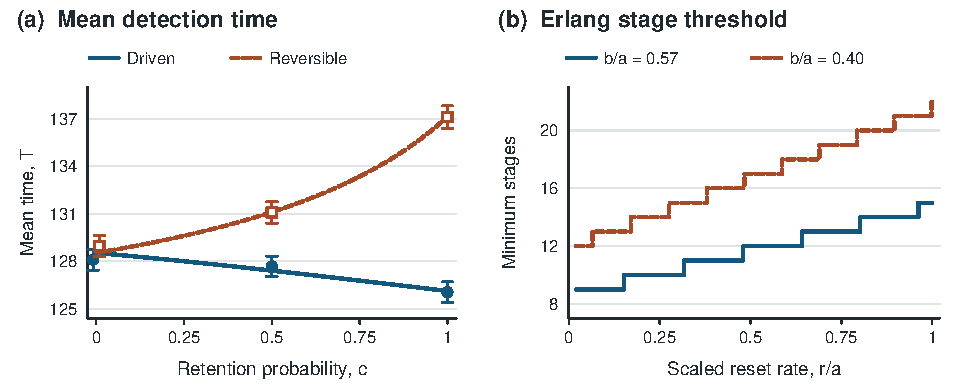
\includegraphics[width=\linewidth]{transport.pdf}
 \caption{Left: mean detection time versus retention for a twelve-state ring, $r=0.2$ and $\tau=4$. Symbols show event-driven means with pointwise 95\% Monte Carlo intervals. Right: minimum number of equal-rate exponential flight stages permitting a strict interior optimum for a three-state ring, after varying the stage rate at fixed $b/a,r/a$.}
 \label{fig:curves}
\end{figure}

In units of the chosen time scale, compare $(k_+,k_-)=(1,0.05)$ with $(0.525,0.525)$. Both have open fraction $1/12$ and jump activity $1.05$. At $c=0$ both give $128.5325$. At $c=1$, (\ref{eq:ring}) gives $126.1270$ for the driven gate and $137.1296$ for the reversible gate. Retention lowers the first mean by $1.87\%$ and raises the second by $6.69\%$. Matching the jump activity controls for the number of internal transitions per unit time. The ordering reflects the temporal correlations of their directions.

We checked these two rings at $c=0,1/2,1$ using three calculations. The Fourier sum (\ref{eq:ring}) and a direct matrix first-step solve agreed to relative tolerance $10^{-12}$. The latter constructs the transition at $\tau$ by Poisson uniformization and separates early resets from flights that missed. For each parameter set we also simulated 150,000 independent trajectories. The reset time was sampled exponentially and the two gate jump counts were sampled as independent Poisson variables, separately before and after a missed crossing. Confidence intervals use the sample standard error times $1.96$. All six intervals contained the analytic value. Scripts, seeds, simulation estimates and interval endpoints accompany this draft. For a direct comparison, the simulated difference $T(1)-T(0)$ was $-2.05$ time units for the driven gate (95\% interval $[-2.96,-1.13]$) and $8.15$ for the reversible gate ($[7.19,9.11]$). Each interval uses the sum of the two independent sample-mean variances. These intervals quantify Monte Carlo uncertainty only.

For an example near the nine-stage boundary, take $a=1$, $b=0.57$, $r=0.1$ and $\kappa=b/\tan(4\pi/27)-(a+r)$. Then $\theta=4\pi/3$ and the derivative phase straddles $3\pi/2$. The two rates $a/3\pm b/\sqrt3$ are strictly positive. The factor $|Z|$ heavily attenuates the signal; evaluating the excess directly in (\ref{eq:three}) avoids subtracting nearly equal large means. Direct solution of the renewal system with 60-decimal arithmetic gives $c_*=0.58709$ and $T(c_*)-T(0)=-3.889\times10^{-11}$ against a baseline $T(0)=5.709\times10^6$. This example establishes attainability; the larger ring in Fig.~\ref{fig:curves} illustrates an effect accessible to trajectory simulation.

\section{A retention window in large driven rings}\label{sec:layer}
Consider a homogeneous $m$-state ring with one open state, rates $k_+>k_->0$,
drift $v=k_+-k_-$ in sites per unit time, and deterministic flight time $\tau$.
As $m$ increases the open fraction $1/m$ decreases. We therefore compare
$D_m(c)=[T(c)-T(0)]/m$ at fixed rates, $\tau$, and $r$.
Put $\delta=r(1-c)$ and write $p_m(t)$ for the return probability on the
ring. The corresponding return probability on the infinite lattice is
\[
 g(t)=e^{-(k_++k_-)t}I_0(2\sqrt{k_+k_-}\,t),
 \qquad H(\tau)=\int_0^\tau g(s)\,ds.
\]
Here $I_0$ is the modified Bessel function. The expression for $g$ follows
by equating independent clockwise and counterclockwise Poisson jump counts.

\paragraph{Proposition 3.}
For fixed $0<c<1$,
\[
 \lim_{m\to\infty}D_m(c)=c\int_0^\infty e^{-\delta s}g(s+\tau)\,ds>0 .
\]
At full retention, $\lim_{m\to\infty}D_m(1)=1/(2v)-H(\tau)$.
For $c_m\in[0,1]$ with $mr(1-c_m)\to z\in(0,\infty)$,
\begin{equation}
 \lim_{m\to\infty}D_m(c_m)=
 F_\tau(z)=\frac{1}{v(1-e^{-z/v})}-\frac{1}{z}-H(\tau).
 \label{eq:ring-layer}
\end{equation}
The continuous extension $F_\tau(0)$ equals the full-retention limit.
There is a unique flight time $\tau_*>0$ satisfying
$H(\tau_*)=1/(2v)$. For $\tau>\tau_*$ the limiting excess is negative at
full retention, although every fixed $0<c<1$ gives positive limiting excess.
Within the scaling in (\ref{eq:ring-layer}) there is a unique $z_*>0$
such that $F_\tau(z)<0$ for $0<z<z_*$ and $F_\tau(z)>0$ for $z>z_*$.

\paragraph{Proof.}
Equation (\ref{eq:main}) gives
$D_m(c)=c\int_0^\infty e^{-\delta s}[p_m(s+\tau)-1/m]\,ds$.
Couple the ring walk to the infinite walk reduced modulo $m$. For fixed $s$
this gives $p_m(s)\to g(s)$, hence the first limit by dominated convergence.
For the other two limits put
$B_m(\delta)=\int_0^\infty e^{-\delta t}[p_m(t)-1/m]\,dt$, including
$\delta=0$ by finite-state mixing. Then, for $c>0$,
\[
 D_m(c)/c=e^{\delta\tau}
 \left[B_m(\delta)-\int_0^\tau e^{-\delta s}[p_m(s)-1/m]\,ds\right].
\]
At $\delta=0$, $B_m(0)$ is a normalized Kemeny trace. Such traces for
driven rings and their reset-induced spectral shifts are studied in
\href{https://arxiv.org/abs/2302.09965}{Mazzolo and Monthus (2023)}.
Writing $A=k_++k_-$, the Fourier modes are
$\lambda(\theta)=-A(1-\cos\theta)+iv\sin\theta$, $\theta=2\pi j/m$.
Taking the real part gives
\[
 B_m(0)=\frac{1}{m}\sum_{j=1}^{m-1}
 \frac{A}{2[v^2+4k_+k_-\sin^2(\pi j/m)]}
 \ \longrightarrow\ \frac{1}{2v}.
\]
The last integral follows by the tangent substitution over a half period.

For $\delta>0$, set $\Delta=\sqrt{(A+\delta)^2-4k_+k_-}$ and
$u_\pm=2k_\pm/(A+\delta+\Delta)$. The infinite-line resolvent from
the origin at site $\ell\ge0$ is $u_+^\ell/\Delta$ and at $-\ell$ is
$u_-^\ell/\Delta$. Indeed these expressions solve the resolvent
recurrence $(A+\delta)G_j-k_+G_{j-1}-k_-G_{j+1}=\mathbf{1}_{\{j=0\}}$
and decay at both ends. Summing the kernel over multiples of $m$ gives
\[
 B_m(\delta)=\frac{1}{\Delta}\left[
 1+\frac{u_+^m}{1-u_+^m}+\frac{u_-^m}{1-u_-^m}\right]
 -\frac{1}{m\delta}.
\]
If $m\delta\to z>0$, then $\Delta\to v$,
$\log u_+=-\delta/v+O(\delta^2)$, and $u_-\to k_-/k_+<1$.
Substitution gives (\ref{eq:ring-layer}). The infinite-line
resolvent at the origin has limit $1/v$ as $\delta\downarrow0$, so
$H$ increases strictly from zero to $1/v$. Finally
$F_\tau'(z)=1/z^2-[4v^2\sinh^2(z/(2v))]^{-1}>0$,
and $F_\tau(+\infty)=1/v-H(\tau)>0$. These observations establish
both threshold statements. \hfill$\square$

For $k_+=1$, $k_-=0.05$, $r=0.5$, $\tau=2$, the
$m=12$ mean drops from $63.23876$ at $c=0$ to $60.57168$ at $c=1$.
The large-ring limit makes an additional prediction. For fixed $c$
below one, even a highly retentive detector eventually loses this advantage;
its mean time exceeds that for a full redraw. At the parameters above, the large-ring curve crosses zero at $z_*=5.263$, whereas the computed finite-ring crossings are $5.937$ and $5.417$ at $m=64$ and $256$, respectively. At $m=256$ the finite-ring crossing corresponds to a refresh probability $1-c=5.417/(256r)=0.0423$. This gives a control setting measurable in the original protocol. Figure~\ref{fig:layer} shows how the sign change approaches the limiting prediction.

\begin{figure}[ht]
 \centering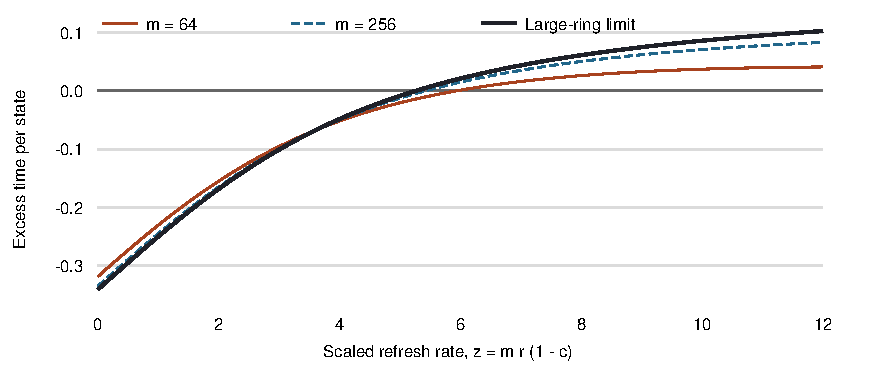
\includegraphics[width=.92\linewidth]{crossover.pdf}
 \caption{Excess mean detection time per gate state against the scaled refresh rate. Negative values favor retention relative to a full redraw. The two finite curves use the exact Fourier sum; the limiting curve uses Eq.~(\ref{eq:ring-layer}). Parameters are $k_+=1$, $k_-=0.05$, $r=0.5$, $\tau=2$.}
 \label{fig:layer}
\end{figure}


\section{Scope and interpretation}
For a three-state detector the advantage of a mixed control policy is limited by damping of the oscillatory mode during flight. A phase lag large enough for an interior minimum also suppresses the magnitude of the corresponding signal. Eq.~(\ref{eq:gainbound}) makes this constraint quantitative. It bounds the savings relative to the faster endpoint, while the twelve-state comparison concerns a change from one endpoint to the other. The gate is observed at an arrival conditioned on the flight surviving a reset. This selects the tilted flight law, and the future reset epochs add exponential averaging. It is the sign of that averaged open-state correlation which governs the advantage of memory. A driven cycle can have a negative correlation in the time window sampled by the detector. Transit-time dispersion shifts and attenuates this window. For a three-state ring the phase accumulated by a sum of exponential transit times is bounded, leading to the stage threshold in (\ref{eq:threshold}).

The model applies to directed transport with one test per launch, independent flight and gate dynamics, and instantaneous resets. Diffusive returns to a closed target, finite dwell times in the sensing region, multiple open states, and feedback from a failed reading change the survival kernel. For an experimental comparison the open fraction, jump activity, reset rate and flight law would need to be controlled separately. The entropy bound assumes a stationary initial gate and known timing law. Neither it nor the predicted speedups have been tested on a physical apparatus.

\paragraph{Code and data.} All numerical observations reported here were generated for the specified models. The accompanying archive includes the simulation and matrix calculations, the stage check, the figure source and the tabulated results.
\paragraph{Use of AI.} OpenAI Codex was used to develop the model analysis, draft the proofs and text, and write and execute the numerical checks. This version is for review by the prospective human authors.

\begin{thebibliography}{9}
\bibitem{bress} P.\ C.\ Bressloff, Diffusive search for a stochastically-gated target with resetting (2020). \href{https://arxiv.org/abs/2009.02739}{arXiv:2009.02739}.
\bibitem{mercado} G.\ Mercado-V\'asquez and D.\ Boyer, Search of stochastically gated targets with diffusive particles under resetting, \emph{J.\ Phys.\ A} \textbf{54}, 444002 (2021). \href{https://doi.org/10.1088/1751-8121/ac27e5}{doi:10.1088/1751-8121/ac27e5}.
\bibitem{biswas} A.\ Biswas, A.\ Pal, D.\ Mondal and S.\ Ray, Rate enhancement of gated drift-diffusion process by optimal resetting (2023). \href{https://doi.org/10.1063/5.0154210}{doi:10.1063/5.0154210}.
\bibitem{scher} Y.\ Scher and S.\ Reuveni, Gated reactions in discrete time and space (2021). \href{https://doi.org/10.1063/5.0072393}{doi:10.1063/5.0072393}.
\bibitem{avra} K.\ Avrachenkov, A.\ Piunovskiy and Y.\ Zhang, Hitting times in Markov chains with restart and their application to network centrality. \href{https://arxiv.org/abs/1503.08548}{arXiv:1503.08548}.
\bibitem{chen} Y.\ Chen, On the monotonicity of autocorrelation function for finite state Markov processes, \emph{Acta Sci.\ Nat.\ Univ.\ Pekin.} \textbf{45} (2009). \href{https://xbna.pku.edu.cn/EN/Y2009/V45/I1/11}{Journal record}.
\bibitem{dechant} A.\ Dechant, J.\ Garnier-Brun and S.-i.\ Sasa, Thermodynamic bounds on correlation times, \emph{Phys.\ Rev.\ Lett.} \textbf{131}, 167101 (2023). \href{https://doi.org/10.1103/PhysRevLett.131.167101}{doi:10.1103/PhysRevLett.131.167101}.
\bibitem{zbik} B. Zbik, B. Dybiec, K. Capała, Z. Palmowski and I. M. Sokolov, Hitting the blinking target under stochastic resetting, \emph{Chaos} \textbf{36}, 043123 (2026). \href{https://doi.org/10.1063/5.0315902}{doi:10.1063/5.0315902}.
\bibitem{barato} A.\ C.\ Barato and U.\ Seifert, Coherence of biochemical oscillations is bounded by driving force and network topology, \emph{Phys.\ Rev.\ E} \textbf{95}, 062409 (2017). \href{https://doi.org/10.1103/PhysRevE.95.062409}{doi:10.1103/PhysRevE.95.062409}.
\end{thebibliography}
\end{document}



